%*****************************************************************
%*************************** Section 6 ***************************
%************************ Bedienungs-Board ***********************
%*****************************************************************


\pagestyle{fancy}
\rhead{\thepage} \chead{} \lhead{\ref{Sec6}. \nameref{Sec6}}
\cfoot{}



\section{Bedienungs-Board}\label{Sec6}

Das Bedienungs-Board ist auf der oberen Fahrzeugebene über dem Controller verbaut. Es enthält ein Display, einen Drehencoder mit Button, einen separaten Button und einen Summer. Diese Komponenten dienen zum einen der Eingabe von Parametern und der Bedienung des Fahrzeugs durch den Benutzer und zum Anderen zum Ablesen der Fahrzeugdaten, wie beispielsweise der Streckenerkennungsdaten der Kamera.

\subsection{Schaltplan}\label{Sec6Sub1}

Das Bedienungs-Board ist eine selbst bestückte Lochrasterplatine, die die Anschlüsse der einzelnen Komponenten auf eine Stiftleiste zusammenführt. In den Abbildungen \ref{fig:BedienungsBoard1} und \ref{fig:BedienungsBoard2} ist der Schaltplan des Bedienungs-Boards zusehen. Die Buchsenleisten J3 und J4 sind die Anschlüsse des Displays. An die Buchsenleisten J5 und J6 sind die Pins des Drehencoders geführt. Dieser gibt zwei Signale (ENC\_A, ENC\_B) für die Erkennung der Drehrichtung und ein Signal (ENC\_SW) für den Taster aus. Die Signale des Displays, des Drehencoders, des Tasters und des Summers werden an die Stiftleisten J1 und J2 geführt, über die die Verbindung zur Controllerplatine hergestellt wird. Die Einbindung des Bedienungs-Boards in das Gesamtsystem des Fahrzeugs ist über den Anhang \glqq{}\nameref{SecAtt1}\grqq{} nachvollziehbar.

\begin{figure}[H] %H für Positionierung hier
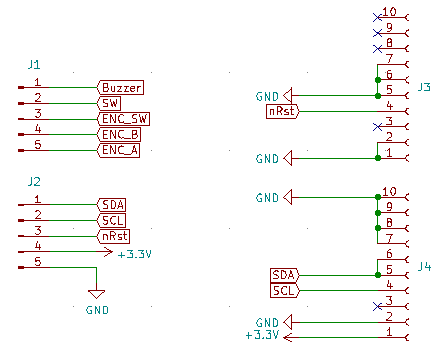
\includegraphics[width=.75\textwidth]{sec6/images/Display_PCB} 
\centering
\captionsetup{width=.95\textwidth}
\caption[Schaltplan des Bedienungs-Boards 1]{Schaltplan des Bedienungs-Boards mit den Stiftleisten J1 und J2 zur Verbindung mit dem Mikrocontroller und den Buchsenleisten J3 und J4 für das Display}\centering
\label{fig:BedienungsBoard1}
\end{figure}

\begin{figure}[H] %H für Positionierung hier
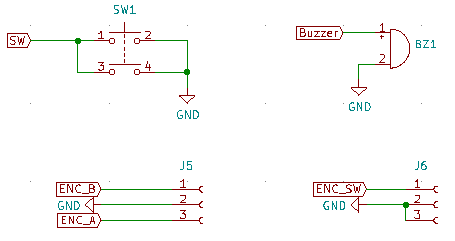
\includegraphics[width=.90\textwidth]{sec6/images/Display_PCB2} 
\centering
\captionsetup{width=.95\textwidth}
\caption[Schaltplan des Bedienungs-Boards 2]{Schaltplan des Bedienungs-Boards mit dem Drehencoder, dem Taster und dem Summer}\centering
\label{fig:BedienungsBoard2}
\end{figure}

\subsection{Programmierung der Steuerelemente}\label{Sec6Sub3}
Die drei Signale des Drehencoders ENC\_A, ENC\_B und ENC\_SW und das Signal SW des Tasters fungieren als Pulldown Anschlüsse. Diese Signale werden im Mikrocontroller über einen internen Pull-Widerstand auf \SI{3,3}{\volt} gezogen. Die beiden Signale ENC\_A und ENC\_B liefern ein Rechtecksignal, dessen Frequenz sich mit der Drehgeschwindigkeit ändert. Durch einen Phasenversatz der beiden Signale um \SI{90}{\degree} kann die Drehrichtung bestimmt werden. Dabei wird bei einer Flanke vom Signal \glqq ENC\_A\grqq{} der Spannungspegel vom Signal \glqq ENC\_B \grqq{} bestimmt. Aus der Information, ob es sich um eine fallende oder steigenden Flanke des Signals ENC\_A handelt und ob der Spannungspegel des Signals ENC\_B \SI{3,3}{\volt} oder \SI{0}{\volt} ist, kann die Drehrichtung und die Anzahl der Schritte bestimmt werden.\\
Das Signal Buzzer lässt bei anlegen einer Spannung den internen Quarz des Summers mit seiner charakteristischen Frequenz schwingen. Dadurch können Eingaben des Benutzers akustisch bestätigt werden.
\begin{figure}[H]	
\centering
	\begin{tikzpicture}[node distance=1.5cm]
		\node (start) [startstop] {Start};
		\node (prInit) [process, below of=start] {counter = 0};
		\node (EncIn)[io, below of=prInit]{Encoder einlesen};
		\node (prENC) [process, below of=EncIn] {Encoder auserten};
		\node (decCounter)[decision,below of=prENC,yshift=-0.5cm]{counter$\geq$10?};
		\node (SWIn)[io,below of = decCounter,yshift=-1cm]{Taster Einlesen};
		\node (prSW) [process, below of=SWIn] {Taster auserten};
		\node (prDelay) [process, below of=prSW] {warte \SI{1}{\milli\second}};
		
		
		\draw [arrow] (start) -- (prInit);
		\draw [arrow] (prInit) -- (EncIn);
		\draw [arrow] (EncIn) -- (prENC);
		\draw [arrow] (prENC) -- (decCounter);
		\draw [arrow] (decCounter) -- node[anchor=east]{ja} (SWIn);
		\draw [arrow] (SWIn) -- (prSW);
		\draw [arrow] (prSW) -- (prDelay);
		
		\draw [arrow](decCounter) -- node[anchor = south]{nein} ++(3,0)|-(EncIn);
		\draw [arrow](prDelay) |- ++(3,-1)--+(0,6.5);
				
	\end{tikzpicture}
	
	\caption[Flussablaufdiagramm Taster und Drehencoder einlesen]{Flussablauf zum Einlesen des Encoders jede Millisekunde und der Taster alle zehn Millisekunden}
	\label{fig:FlussablaufEncTaster}
\end{figure}
\subsubsection{Taster auswerten}\label{sec:Taster}
Im Flussablaufdiagramm in Abbildung \ref{fig:FlussablaufEncTaster} werden die beiden Taster mit einer Abtastzeit von \SI{10}{\milli\second} eingelesen. Da Taster mechanische Bauteile sind kommt es bei jedem Betätigen zu ungewollten Pegelwechseln, dem sogenannten Prellen. Dies muss verhindert werden, da dadurch ein Tastendruck als mehrere interpretiert werden kann. Soll zum Beispiel ein Zähler per Tastendruck um eins inkrementiert werden, wird bei einem prellendem Taster der Zähler pro Druck nicht um eins erhöht sondern um zum Beispiel fünf. Die Anzahl um wie viel der Zähler erhöht wird hängt davon ab, wie viele Pegelwechsel durch das Prellen erzeugt wird und mit welcher Frequenz der Taster ausgelesen wird. Um das Prellen zu verhindern können spezielle prellfreie Taster verwendet werden, da diese recht teuer sind und der Taster im Drehencoder nicht ausgetauscht werden kann, wird auf eine softwareseitige Entprellung zurückgegriffen. Dabei wird ein Tastendruck nur erkannt, wenn sich der Spannungspegel des Tasters für vier Abtastzyklen nicht ändert. Dies entspricht bei einer Abtastzeit von \SI{10}{\milli\second} einer Zeit von \SI{40}{\milli\second}. Bei diesem verfahren ist wichtig, dass der Taster mindestens die vierfache Zeit der Abtastzeit gedrückt wird. Beim Entprellen wird zuerst abgefragt, ob sich der eingelesene Zustand des Tasters zum vorherigen entprellten Zustand geändert hat. Ist dies der Fall wird ein Zähler dekrementiert. Der Zähler zählt von drei bis null. Erreicht dieser den Wert null oder wird ein Zustand eingelesen, der dem zuvor entprelltem Zustand entspricht, wird der Zähler auf den Wert drei zurückgesetzt. Wechselt der Zähler von null auf drei, wird der Tastendruck als solcher erkannt. \\\\Im C-Code wird der Zähler mit zwei 32 Bit Variablen implementiert. Dabei wird aus jeweils einem Bit der beiden Variablen ein zwei Bit Zähler gebildet. Dadurch entstehen mit nur zwei Variablen insgesamt 32 Zähler, die von drei bis null zählen können. Dies macht jedoch die Implementierung der Zählfunktion schwieriger, da der Zähler nicht mit einem Postdekrement und if-Abfragen realisiert werden kann. Diese Funktionen müssen durch Bitoperationen ersetzt werden, die die ganze 32 Bit variable abfragen und ändern können (siehe ...).

\subsubsection{Drehencoder auswerten}\label{sec:Drehencoder}
Im Flussablaufdiagramm in Abbildung \ref{fig:FlussablaufEncTaster} werden die beiden um \SI{90}{\degree} Phasenverschobenen Signale des Drehencoders mit einem Zeitabstand von \SI{1}{\milli\second} ausgelesen. Im Anschluss darauf müssen daraus die Drehrichtung und die Anzahl der gedrehten Schritte ermittelt werden. Dazu wird in einer Variable der aktuell gemessene und der jeweils letzte Wert der beiden Drehencoder Anschlüsse als je ein Bit gespeichert. Dabei liegt in Bit0 der aktuelle Zustand von ENC\_B, in Bit1 der aktuelle Zustand von ENC\_A, in Bit2 der letzte Zustand von ENC\_B und in Bit3 der letzte Zustand von ENC\_A. Die daraus entstehende vier Bit große Zahl bildet den Index eines Array, das Anzeigt, ob der Drehencoder nach links oder nach rechts gedreht wird. Steht in der Variable zum Beispiel der Wert 1101\textsubscript{2} (13\textsubscript{10}) bedeutet das, dass die vorherigen Zustände beide eins waren, der aktuelle Zustand von ENC\_A LOW und der von ENC\_B HIGH ist. Daraus ist abzuleiten, dass eine fallende Flanke des Signals ENC\_A und ein HIGH Pegel am Signal ENC\_B anliegt. In dem Array an der Stelle 13 steht der Wert -1, was eine Drehung im Uhrzeigersinn darstellt. Im Falle von 1000\textsubscript{2} (8\textsubscript{10}) liegt eine fallende Flanke an ENC\_A und ein LOW Pegel an ENC\_B an. Daraus ergibt sich im Array der Wert 1 an der Stelle acht, was eine Drehrichtung gegen den Uhrzeigersinn darstellt.
\newpage
\subsection{Programmierung der Anzeige}\label{Sec6Sub2}
Für die Anzeige von Fahrzeugparametern wird ein 64 mal 128 Pixel großes \ac{OLED} verwendet, dessen Ansteuerung über eine \ac{I2C} Schnittstelle erfolgt.  Mit dem Pin 6 von J3 wird die \ac{I2C} Adresse auf 3C\textsubscript{16} (GND) oder 3E\textsubscript{16} (\SI{3,3}{\volt}) festgelegt. Dem Schaltplan in Abbildung \ref{fig:BedienungsBoard1} kann entnommen werden, dass die Adresse auf 3C\textsubscript{16} festgelegt ist. Außerdem wird das Reset Signal des Controllers an den Pin 4 der Stiftleiste J3 angelegt.

\subsubsection{Funktionsweise des \acl{OLED}s}\label{sec:FunktionOLED}
Auf der Platine des Displays ist der Displaycontroller SSD1309 von SOLOMON SYSTECH verbaut. Dieser Kommuniziert mit dem Mikrocontroller und steuert die Segment- und COM-Anschlüsse des Displays an. Das Display besitzt 64 COM-Anschlüsse für die Kathoden der LEDs und 128 Segmentanschlüsse für die Anoden der LEDs. Jeder COM-Anschluss entspricht einer Zeile des Displays und jeder Segmentanschluss einer Spalte (siehe Schaltplan in Abbildung \ref{fig:OLEDSchaltplan}). Somit kann durch Auswahl einer Reihe mit einem COM-Anschluss und durch Ansteuern des Segmentanschluss, jedes Pixel angesprochen werden. Im Displaycontroller ist ein \ac{RAM} mit 64 Zeilen und 128 Spalten verbaut. Jeder Zeile des Speichers ist eine Zeile (COM-Anschluss) des Displays und jeder Spalte des Speichers ist eine Spalte des Displays (Segmentanschluss) zugeordnet. Somit ist jedem Bit im \ac{RAM} ein Pixel auf dem Display zugewiesen. Acht Zeilen des Speichers werden zu einer Seite zusammengefassst. Bit null eines Wertes entspricht der ersten Zeile der Seite und Bit sieben der achten Zeile. Ein Bild auf dem Display wird aufgebaut indem zuerst das Segment SEG0 mit einem HIGH Pegel ausgewählt wird und die ersten acht im \ac{RAM} gespeicherten Pixelwerte an den Anschlüssen COM0 bis COM7 angelegt werden. Danach wird das Segment SEG1 ausgewählt und die zweiten acht Pixelwerte an die gleichen COM-Anschlüsse angelegt. Diese wird bis zum letzten Segment fortgeführt. Ist dies erreicht wird wieder das Segment SEG0 ausgewählt. Diesmal werden die Pixelwerte jedoch an die Anschlüsse COM8 bis COM15 angelegt. Nach dem das letzte Segment und die letzten acht COM-Anschlüsse angesteuert wurden, beginnt der Durchlauf von vorn. In den Einstellungen des Displaycontroller kann eingestellt werden von welcher Startseite bis zu welcher Stopseite die COM-Anschlüsse angesteuert werden. Dadurch können Seiten am oberen und unteren Rand ausgelassen und somit der Displaybereich eingegrenzt werden. Das Start- und Stoppsgement kann ebenfalls bestimmt werden und somit der rechte und linke Displayrand beschränkt werden. Außerdem kann die horizontale Orientierung festgelegt werden, in dem man die Zuordnung des Segments null auf die Speicherspalte null oder 127 legt. Dadurch werden die ersten Pixelwerte im Speicher nicht in die Spalte des Segments SEG0 sondern in die Spalte vom Segment SEG127. Die Einstellung der vertikale Orientierung erfolgt mit der Richtung, mit der die Zeilen des Speichers auf die COM-Anschlüsse gelegt werden.
\begin{figure}[H]
\begin{circuitikz}
\draw 	(0,0)node[anchor=south]{SEG0}to[short,o-*](0,-1) to[led,-*] (0,-3)
		(2,0)node[anchor=south]{SEG1}to[short,o-*](2,-1) to[led,-*] (2,-3)
		(4,-2)node[circ]{}
		(5,-2)node[circ]{}
		(6,-2)node[circ]{}
		(8,0)node[anchor=south]{SEG127}to[short,o-*](8,-1) to[led] (8,-3)
				
		(1,-3)node[jump crossing](j00){}
		(3,-3)node[jump crossing](j10){}
		
		(-1,-3)node[anchor=east]{COM0}to[short,o-](j00.west) 
		(j00.east)--(j10.west)
		(j10.east)--(3.5,-3)
		(7.5,-3)--(8,-3)

		(0,-4)to[led,-*] (0,-6) (0,-1)-|(j00.north)(j00.south)to[short,-*](1,-4)--(0,-4)
		(2,-4)to[led,-*] (2,-6)	(2,-1)-|(j10.north)(j10.south)to[short,-*](3,-4)--(2,-4)
		(4,-5)node[circ]{}
		(5,-5)node[circ]{}
		(6,-5)node[circ]{}
		(8,-4)to[led] (8,-6)	(8,-1)--(9,-1)to[short,-*](9,-4)--(8,-4)
		
		(1,-6)node[jump crossing](j01){}
		(3,-6)node[jump crossing](j11){}		
			
		(-1,-6)node[anchor=east]{COM1}to[short,o-](j01.west) 
		(j01.east)--(j11.west)
		(j11.east)--(3.5,-6)
		(7.5,-6)--(8,-6)
		
		(1,-4)--(j01.north)	(j01.south)--(1,-6.5)
		(3,-4)--(j11.north)	(j11.south)--(3,-6.5)
		(9,-4)--(9,-6.5)
		
		
		(0,-7)node[circ]{}
		(0,-7.5)node[circ]{}
		(0,-8)node[circ]{}
		
		(2,-7)node[circ]{}
		(2,-7.5)node[circ]{}
		(2,-8)node[circ]{}
		
		(8,-7)node[circ]{}
		(8,-7.5)node[circ]{}
		(8,-8)node[circ]{}
		
		
		(0,-9)to[led,-*] (0,-11) 	%(0,-1)-|(j00.north)(j00.south)to[short,-*](1,-4)--(0,-4)
		(2,-9)to[led,-*] (2,-11)	%(2,-1)-|(j10.north)(j10.south)to[short,-*](3,-4)--(2,-4)
		(4,-10)node[circ]{}
		(5,-10)node[circ]{}
		(6,-10)node[circ]{}
		(8,-9)to[led] (8,-11)		%(8,-1)--(9,-1)to[short,-*](9,-4)--(8,-4)
		
	
		
		(-1,-11)node[anchor=east]{COM63}to[short,o-](3.5,-11)(7.5,-11)--(8,-11)
		(0,-9)-|(1,-8.5)
		(2,-9)-|(3,-8.5)
		(8,-9)-|(9,-8.5)	
;

\draw[dotted]
	(3.5,-3)--(7.5,-3)
	(3.5,-6)--(7.5,-6)
	(3.5,-11)--(7.5,-11)

	(1,-6.5)--(1,-8.5)
	(3,-6.5)--(3,-8.5)
	(9,-6.5)--(9,-8.5)
;
\end{circuitikz}
\caption[Schaltplan OLED]{Repräsentativer Schaltplan des \acp{OLED} mit Segment- und COM-Anschlüssen}
\label{fig:OLEDSchaltplan}
\end{figure}

\subsubsection{I2C Ansteuerung}\label{sec:OLEDI2C}
%i2c_rtos_interface.c
%ssd1309.c
%ssd1309_rtos.c

Die Kommunikation mit dem \ac{OLED} erfolgt mit einer \ac{I2C} Schnittstelle. Dazu wird auf dem Mikrocontroller ein sogenanntes Flexcomm Modul verwendet. Diese Module besitzen mehrere Schnittstellen wie zum Beispiel UART, SPI oder \ac{I2C}. Zu beginn wird der Pin 3.24 als SCL und der Pin 3.25 als SDA des Flexcomm2 Moduls konfiguriert. Danach wird das Modul selbst mit der Funktion \glqq I2C\_MasterInit\grqq{} von NXP so initialisiert, dass die Taktfrequenz des SDA Signals ca. \textcolor{red}{\SI{333}{\kilo\hertz}} beträgt. Dabei ist das Problem entstanden, dass das Modul zuerst keine Daten sendet. Nach dem Debuggen und überprüfen jedes Registers des Moduls wird festgestellt, dass der Takt für das Modul deaktiviert ist. Dies ist ärgerlich, da bei der Konfiguration auf Funktionen zurückgegriffen wird, die von NXP stammen. Nach dem der Takt für das Flexcomm2 Modul aktiviert ist werden die Daten wie gewünscht über die Schnittstelle gesendet.\\\\ Um den Prozessor zu entlasten wird auf die zusendenden Daten per \ac{DMA} zugegriffen. Dadurch werden diese parallel zum Prozessor in das Senderegister des Flexcomm2 Moduls geladen und der Prozessor wird nicht mit einfachem hin- und herschieben von Daten aufgehalten. Zu aller erst wird das \ac{DMA} Modul DMA0 mit der von NXP zur Verfügung gestellten Funktion \glqq DMA\_Init\grqq{} initialisiert. Dem Datenblatt kann in Tabelle 300 entnommen werden, dass der Kanal fünf mit der \ac{I2C} Funktion des Flexcomm2 Moduls verbunden ist. Deshalb wird mit der ebenfalls Bereitgestellten Funktion \glqq DMA\_EnableChannel \grqq{} der Kanal fünf freigegeben. Dann wird mit den beiden Funktionen \glqq DMA\_CreateHandle\grqq{} und \glqq I2C\_MasterTransferCreateHandleDMA\grqq{} die Funktionalität des \ac{DMA}s mit dem Flexcomm2 Modul freigegeben.\\\\ Jetzt kann mit der Funktion \glqq I2C\_MasterTransferNonBlocking\grqq{} eine Übertragung über \ac{I2C} und \ac{DMA} begonnen werden. Dieser Funktion wird in einer Variable ein Pointer auf die zusendende Variable und deren Länge übergeben. Sollen anzuzeigende Daten and das \ac{OLED} übertragen werden wird der Funktion ein Pointer auf einen zuvor definierten Speicherbereich und dessen Länge übergeben. Soll eine Konfiguration gesendet werden, muss der Funktion ein Pointer auf eine acht Bit große Variable und die Länge eins übergeben werden. Die Übergabe in die Funktion erfolgt mit einer \glqq struct\grqq{} Variable, die neben dem Pointer und der Länge noch die Slaveadressse des Displays, eine Variable für die Richtung der Übertragung, ob es sich um eine Konfiguration oder um Daten handelt und wie die Start- und Stopbits gesendet werden. Die Auswahl, ob es sich um eine Konfiguration handelt oder nicht erfolgt über die sogenannte Subadresse diese wird nach der Slaveadresse übertragen. Deshalb muss der Funktion ebenfalls die Länge der Subadresse übergeben werden.

\subsubsection{Konfiguration des Displays}
Zu Beginn werden einige Resetparameter (siehe Tabelle \ref{tab:InitOLED})übertragen, die das Display zuerst ausschalten und den Kontrast einstellen. Danach wird ein Kommando gesendet, das den Speicher des \ac{OLED} Controllers so einstellt, dass dessen Inhalt eins zu eins auf dem Display angezeigt wird. Eine andere Möglichkeit wäre hier, dass der Inhalt des \ac{RAM}s ignoriert wird. Das Display wird im normalem Modus gestartet. Dies bedeutet, dass eine eins im Speicher die Pixel einschaltet. Im Falle des horizontalen Modus wird das Bild, das auf dem Display angezeigt werden soll wie im Kapitel \ref{sec:FunktionOLED} aufgebaut. Der Befehl 40\textsubscript{16} bestimmt die Zeile des Displays welche dem Anschluss COM0 zugewiesen wird. Durch ändern dieses Wertes kann der Inhalt des Displays nach oben beziehungsweise unten geschoben werden. Mit dem nächsten Kommando wird die horizontale Orientierung eingestellt. In diesem Fall wird der Inhalt des Speichers von Segment 127 nach Segment null ausgegeben. Mit dem Befehle \glqq scan from COM N-1 to COM0\grqq{} wird die vertikale Orientierung verändert. Wobei N dem \glqq MUX ratio\grqq{} (Anzahl der COM-Anschlüsse) entspricht. Die Hardware der COM Pins wird auf ihren Reset Wert gestellt, was bedeutet dass die geraden Zeilen mit den ersten 32 COM-Anschlüssen und die ungeraden mit den restlichen 32 COM-Anschlüssen verbunden ist. Danach werden die GPIO Pins als Eingänge konfiguriert. Das nächste Kommando stellt die Frequenz, des Displays auf ihren korrekten Wert. Außerdem wird die Anzahl der Takte in Phase 1 und Phase 2 auf jeweils zwei Takte gestellt. In Phase 1 wird die Spannung des Pixels entladen und in Phase 2 auf ihren neuen Wert aufgeladen. Diese Werte müssen den Kapazitätswerten der Pixel angepasst werden. Das letzte Kommando stellt die Spannung bezogen auf die Versorgungsspannung des Displays ein, wenn die COM-Anschlüsse deaktiviert sind.
\begin{table}[H]
\centering
	\begin{tabular}{|c|l||c|l|}
	\hline
	AE&Display off&A8&set MUX ratio to\\
	&&3F&64MUX\\
	\hline
	81&Contrast Controll&C8&scan from COM N-1\\
	7F&&&to COM 0\\
	\hline
	A4&display on, output RAM content&D3&no vertical shift\\
	&&00&\\
	\hline
	A6&Normal display mode&DA&set COM pins\\
	&&12&hardware to reset\\
	\hline
	20&Horizontal mode&DC&GPIO pins are inputs\\
	00&&02&\\
	\hline
	21&set column address&D5&increace F\textsubscript{OSC} frequency\\
	00&start address&F0&\\
	7F&end address&&\\
	\hline
	22&set page address&D9&Phase 1 and 2 period to reset\\
	00&to reset value&22&\\
	07&&&\\
	\hline
	40&set display start&DB&set V\textsubscript{COMH} to $0.78 \cdot V_{cc}$\\
	&line to top line&34&\\
	\hline
	A1&column address 127&&\\
	&is SEG0&&\\
	\hline
	\end{tabular}
	\caption[Initialisierungswert \ac{OLED}]{Werte, die der Reihe nach über \ac{I2C} zum \ac{OLED} gesendet werden}
	\label{tab:InitOLED}
\end{table}
Nach der Reset Konfiguration muss noch die Konfiguration erfolgen, die für die Anwendung auf dem Fahrzeug passend ist. Dazu wird die horizontale Orientierung so verstellt, dass die Spaltenadresse 127 im Speicher dem Segment SEG127 entspricht. Ebenso wird die vertikale Orientierung auf den Wert eingestellt, dass das Display von den COM-Anschlüssen COM0 nach COM64 angesteuert werden. Danach wird das Display eingeschaltet.
\subsection{Darstellungen auf dem \acl{OLED}}\label{sec:OLEDDarstellen}
Die im Folgenden genannten Funktionen werden zur Darstellung von Formen und Text beziehungsweise Zahlen verwendet. Beim Aufruf einer dieser Funktionen wird eine Variable gesetzt, die anzeigt, dass dem \ac{OLED} neue Daten geschickt werden müssen. In einem Echtzeittask wird diese alle \SI{30}{\milli\second} geprüft und wenn notwendig die neuen Daten gesendet. 
\subsubsection{Pixelansteuerung}\label{sec:OLEDPixel}
Mit der Funktion \glqq ssd1309\_set\_pixel\grqq{} wird ein Pixel an einer vorgegebenen Position gesetzt oder gelöscht. Dabei wird das anzusprechende in der globalen Variable für den Displaypuffer gesetzt oder gelöscht.
\subsubsection{Rechteck zeichnen}\label{sec:OLEDRect}
Zum Darstellen von Rechtecken wird die Funktion \glqq ssd1309\_draw\_rect\grqq{} verwendet. Dieser werden die Koordinaten der linken oberen und rechten unteren Ecke, eine Variable die angibt ob das Rechteck ausgefüllt ist oder nur der Rand angezeigt werden soll. Außerdem muss angegeben werden, ob die Pixel des Rechtecks angezeigt oder gelöscht werden sollen. In der Funktion werden mit zwei Schleifen alle Pixel innerhalb des Rechtecks durchgegangen und für jeden Pixel bestimmt, ob dieser angezeigt werden soll oder nicht. Soll das Pixel angezeigt werden, wird mit der Funktion \glqq ssd13099\_set\_pixel\grqq{} aus Kapitel \ref{sec:OLEDPixel} dargestellt.
\subsubsection{Buchstabe darstellen}\label{sec:OLEDBuchstabe}
Der Funktion \glqq ssd1309\_write\_char\grqq{} wird eine char Variable übergeben, die am Display angezeigt werden soll. In \glqq struct\grqq Variablen mit dem Namen \glqq ssd1309\_font\_t\grqq{} sind für alle darstellbaren Buchstaben und Zeichen Werte hinterlegt, die diese in unterschiedlichen Größen darstellen. In der Funktion selbst wird zu beginn überprüft, ob der übergebene Charakter ein darstellbares Ascii-Zeichen ist. Ist die der Fall muss abgefragt werden ob das Zeichen innerhalb des Displays liegt. Wenn ja wird mit zwei Schleifen jedes Pixel innerhalb der Höhe und Breite des Zeichens geprüft, ob dieses angezeigt werden soll. Pixel, die angezeigt werden, werden mit der Funktion \glqq ssd1309\_set\_pixel\grqq{} aus Kapitel \ref{sec:OLEDPixel} dargestellt. Die Position wird über einen Cursor eingestellt, der vor Funktionsaufruf gesetzt werden muss.
\subsubsection{Text darstellen}\label{sec:OLEDText}
Die Funktion \glqq ssd1309\_write\_str\grqq{} stellt am Display einen Text dar, der mit einem Pointer auf ein Charakterarray übergeben wird. Da in der Funktion die Funktion \glqq ssd1309\_write\_char\grqq{} in einer Schleife, die sooft ausgeführt wird, wie viele Elemente das Array hat, verwendet wird, muss der Funktion zum Darstellen eines Textes auch die Höhe und Breite der Zeichen in Form von einer \glqq ssd1309\_font\_t\grqq{} Variablen übergeben werden. Die Position des Textes wird wie bei den Buchstaben über den Cursor eingestellt, der vor Funktionsaufruf gesetzt werden muss.
\subsubsection{Bilder darstellen}\label{sec:OLEDBild}
Die Funktion \glqq ssd1309\_draw\_img\grqq{} stellt Bilder dar, die als Hexadezimal Wert abgespeichert sind. Die Position der linken oberen Ecke muss der Funktion übergeben werden. Das Bild selbst wird in einer \glqq struct\grqq{} Variable mit dem Namen \glqq ssd1309\_img\_t\grqq{} übergeben, die ebenfalls die Breite und Höhe des Bildes enthält. Angezeigt wird das Bild mit zwei Schleifen, in denen jedes Pixel überprüft wird, das angezeigt werden soll. Dargestellt werden die einzelnen Pixel mit der Funktion \glqq ssd1309\_set\_pixel\grqq{} aus Kapitel \ref{sec:OLEDPixel}.
\subsection{Menuführung}\label{sec:OLEDMenu}
Der Mikrocontroller muss die Menüführung auf Basis der Werte des Drehencoders und der beiden Taster vornehmen. Ein Zustandsautomat entscheidet je nach dem ob der Hauptbildschirm oder ein Menü angezeigt wird, was die einzelnen Bedienelemente bewirken. Bevor der Zustandsautomat ausgeführt werden kann, müssen die beiden Zustände der entprellten Taster sowie die Anzahl der Schritte, die der Drehencoder in welch Richtung gemacht hat, gespeichert werden. Der Zustandsautomat berechnet alle \SI{20}{\milli\second} das aktuelle Menü und ändert den Displaypuffer ab, sodass das aktuelle Menü dargestellt wird.\\
Es gibt insgesamt vier verschieden Arten von Menüs.
\begin{itemize}
\item MENU\_LINK
\item MENU\_CHECK
\end{itemize}





\newpage